% monster ability cards and initiative tokens

\documentclass{article}
\usepackage[paperwidth=200mm,width=200mm,height=400mm,paperheight=400mm]{geometry}
\pagestyle{empty}
\usepackage{tikz}
\usetikzlibrary{calc}
\def\stride{15.4}
\def\leftcard{12}
\begin{document}
\vbox{\bigskip}
\begin{center}
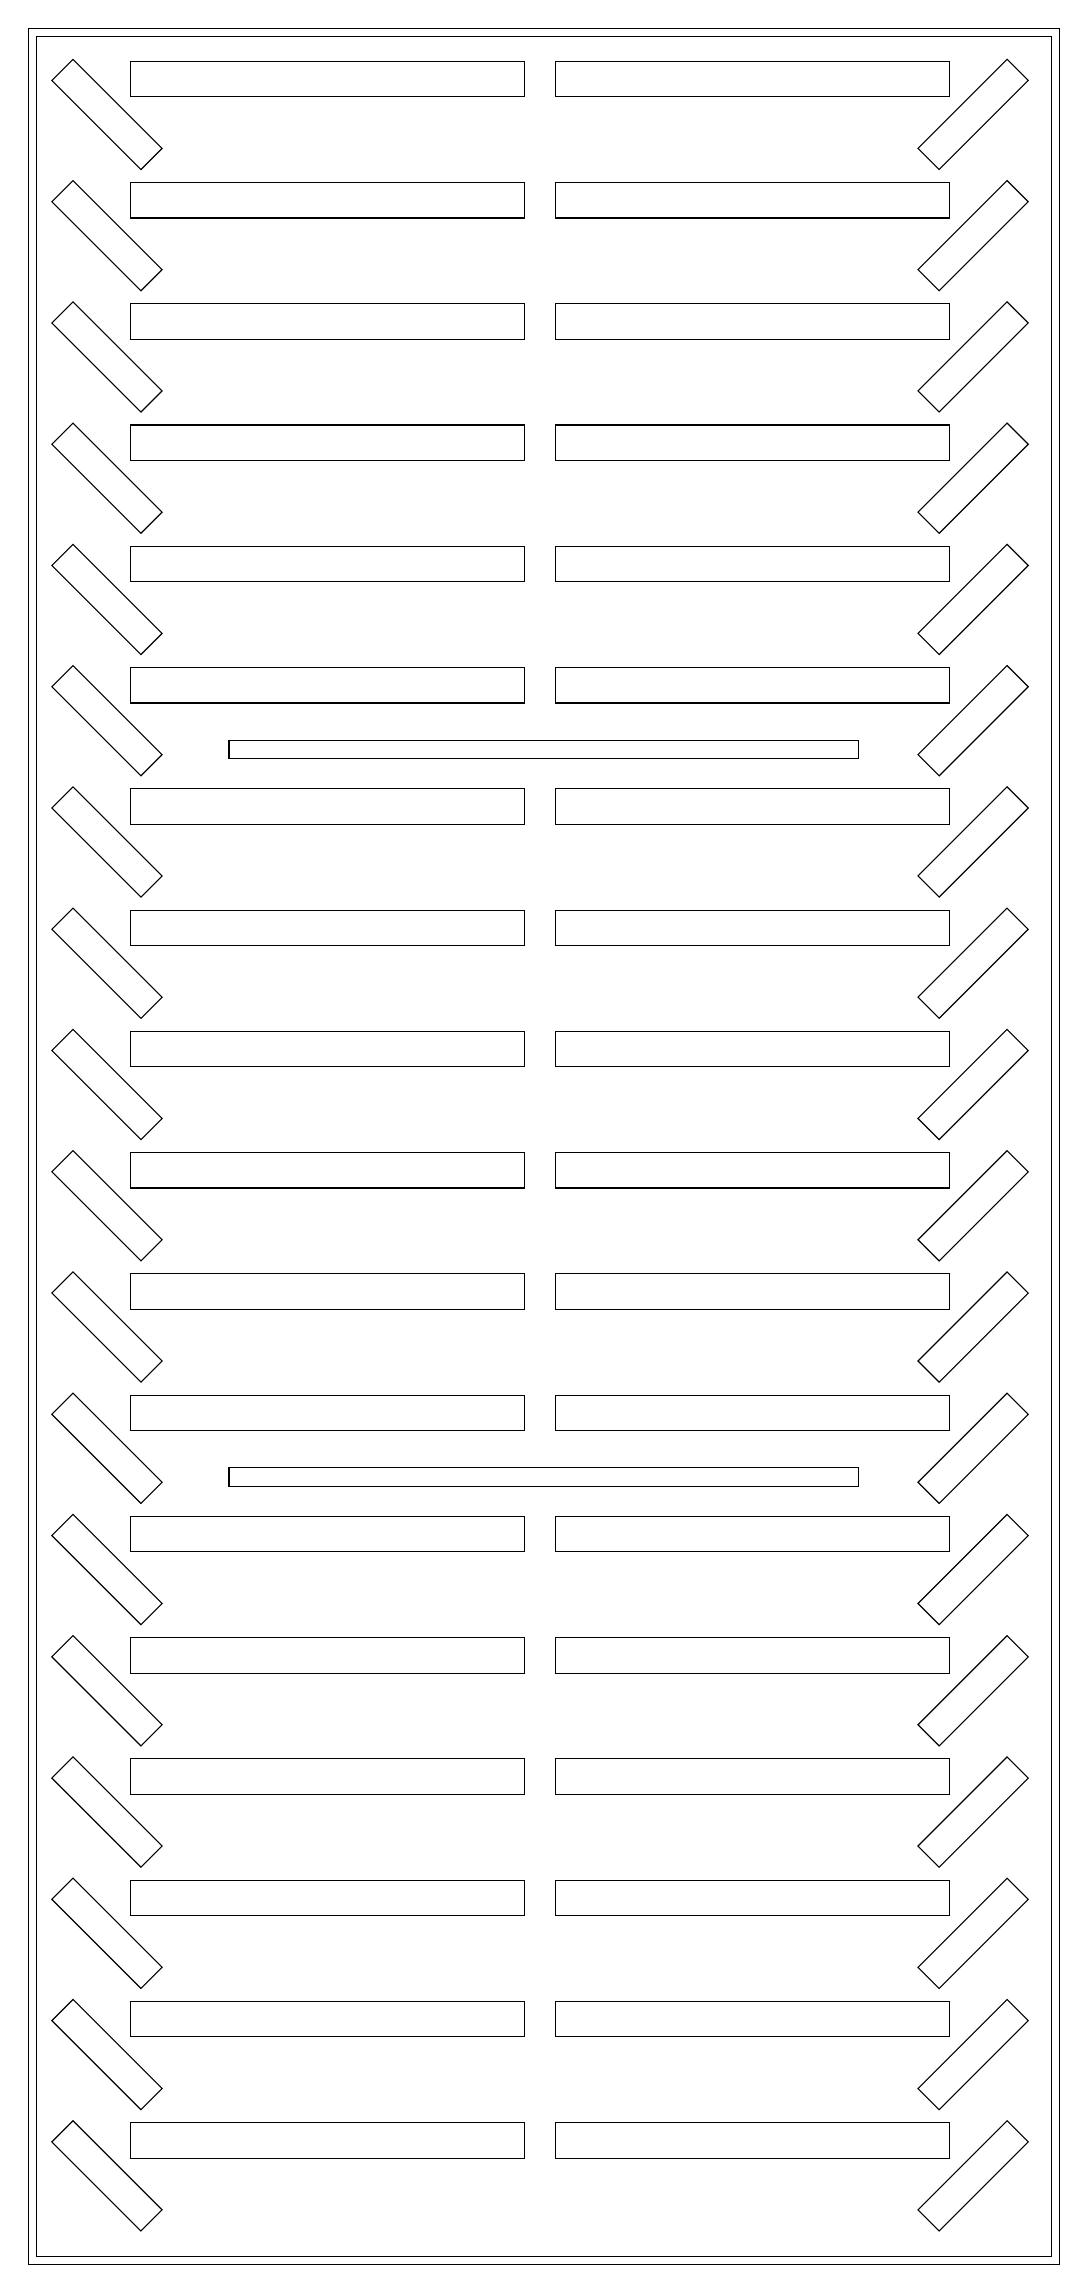
\begin{tikzpicture}[x=1mm,y=1mm]
\draw (-1,-1) rectangle +(131,284);
\draw (0,0) rectangle +(129,282);
\foreach \i in {0,...,17} {
  \draw ($(\leftcard,\i*\stride+12.5)$) rectangle +(50mm,4.5mm);
  \draw ($(\leftcard+54,\i*\stride+12.5)$) rectangle +(50mm,4.5mm);
}
\foreach \i in {0,...,17} {
  \draw ($(9,\i*\stride+6+4.25)$) node[rotate=-45,minimum width=16mm,minimum height=3.8mm,draw] { };
  \draw ($(9+110,\i*\stride+6+4.25)$) node[rotate=45,minimum width=16mm,minimum height=3.8mm,draw] { };
}
\foreach \i in {1,2} {
  \draw ($(64.5,\i*6*\stride+0.3*\stride+2)$) node [minimum height=2mm,minimum width=80mm,draw]{};
}
\end{tikzpicture}
\end{center}
\end{document}
